\documentclass[12pt]{article}
\usepackage[margin=2.5cm]{geometry}
\usepackage{enumerate}
\usepackage{amsfonts}
\usepackage{amsmath}
\usepackage{fancyhdr}
\usepackage{amsmath}
\usepackage{amssymb}
\usepackage{amsthm}
\usepackage{mdframed}
\usepackage{graphicx}
\usepackage{subcaption}
\usepackage{adjustbox}
\usepackage{listings}
\usepackage{xcolor}
\usepackage{courier}
\usepackage[utf]{kotex}
\usepackage{hyperref}
\usepackage{soul}

\definecolor{codegreen}{rgb}{0,0.6,0}
\definecolor{codegray}{rgb}{0.5,0.5,0.5}
\definecolor{codepurple}{rgb}{0.58,0,0.82}
\definecolor{backcolour}{rgb}{0.95,0.95,0.92}

\lstdefinestyle{mystyle}{
    backgroundcolor=\color{backcolour},
    commentstyle=\color{codegreen},
    keywordstyle=\color{magenta},
    numberstyle=\tiny\color{codegray},
    stringstyle=\color{codepurple},
    basicstyle=\ttfamily\footnotesize,
    breakatwhitespace=false,
    breaklines=true,
    captionpos=b,
    keepspaces=true,
    numbers=left,
    numbersep=5pt,
    showspaces=false,
    showstringspaces=false,
    showtabs=false,
    tabsize=1
}

\lstset{style=mystyle}

\pagestyle{fancy}
\renewcommand{\headrulewidth}{0.4pt}
\lhead{CSC 369}
\rhead{Midterm 5 Solution}

\begin{document}
\title{CSC 369 Midterm 5 Solution}

\bigskip

\begin{enumerate}[1.]
    \item

    No. if the access is read for both threads, then concurrency error will not occur.

    \item

    \texttt{b)}, \texttt{c)} and \texttt{d)} are true

    \bigskip

    \begin{mdframed}
    \underline{\textbf{Correct solution}}

    \bigskip

    \texttt{c)} and \texttt{d)} are true
    \end{mdframed}

    \bigskip

    \underline{\textbf{Notes}}

    \begin{itemize}
        \item [\color{blue}Question\color{black}] What does it mean when mutex is held by this thread?
        \item [\color{blue}Question\color{black}] What I do know is that \texttt{pthread\_cond\_wait}
        puts thread to sleep. My question here is, how come the mutex is not held when thread is in a blocked state/sleep?
    \end{itemize}

    \item

    \begin{enumerate}[a)]
        \item

        Only \texttt{b)} causes starvation.

        \item

        Conditional variable is a queue that allows threads to be put themselves on to
        sleep (in blocked state) when thread it is not desired using \texttt{pthread\_cond\_wait}
        function.

        \bigskip

        Since there are no threads inside \texttt{cv1}, there is nothing to awake using
        \texttt{pthread\_cond\_signal}.

        \bigskip

        So, nothing will occur.

        \bigskip

        \item

        System call is a subset of interrupt caused by user application to switch
        from user mode to kernel mode to perform previleged operations for the application.

        \bigskip

        Interrupt is a signal sent by hardware (e.g keyboard, mouse, hard drive) or software.

        \bigskip

        It tells the cpu to stop its activities and execute appropriate part of the operating system.

        \bigskip

        \underline{\textbf{Notes}}

        \begin{itemize}
            \item I need to review how interrupt works. I had to look up the information.
            \item [\color{blue}Question\color{black}] How does interrupt work?
            \item \textbf{Interrupt}

            \bigskip

            \begin{center}
            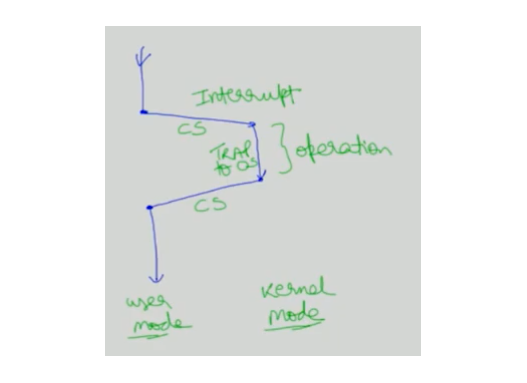
\includegraphics[width=0.8\linewidth]{../../images/midterm_5_solution_1.png}
            \end{center}
        \end{itemize}

        \item

        No. This statment is false.

        \bigskip

        User level threads are generated in user-mode without kenerel being aware about it.

        \bigskip

        \bigskip

        \underline{\textbf{Notes}}

        \begin{itemize}
            \item [\color{blue}Question\color{black}] What is the difference between user-level thread
            and kernel-level thread?
            \item [\color{blue}Question\color{black}] Why is thread that is generated at user level using procedure
            call faster than kernel level thread?
            \item [\color{blue}Question\color{black}] What is procedure call? How does it work?
        \end{itemize}

        \item

        System calls do not generate processes. \texttt{fork()} does.

        \bigskip

        With this reason the program \texttt{run\_stuff} generates only 1 additional process.

        \bigskip

        \underline{\textbf{Notes}}

        \begin{itemize}
            \item [\color{blue}Question\color{black}] What is a process? And how does process work?
            \item [\color{blue}Question\color{black}] How come system call doesn't generate process? And how come
            fork() generates process?

            \item \textbf{Process}

            \begin{itemize}
                \item Is a running program
                \item Has 3 states
                \begin{enumerate}[1.]
                    \item \textbf{Running:}
                    \begin{itemize}
                        \item means a processs is running on a processor
                        \item means instructions are being executed
                    \end{itemize}
                    \item \textbf{Ready:}
                    \begin{itemize}
                        \item means a process is ready to run
                        \item means OS has chosen not to run the program at the given moment
                    \end{itemize}
                    \item \textbf{Blocked:}
                    \begin{itemize}
                        \item means a process has performed some kind of operation that makes it not ready to run
                        until some event takes place
                    \end{itemize}
                \end{enumerate}
            \end{itemize}
        \end{itemize}
    \end{enumerate}
\end{enumerate}

\end{document}